\begin{table*}[!t]
\centering
\small
\setlength{\tabcolsep}{3pt}
\caption{Published solvers and frozen deployment at nominal $T=5$: within-family mean objective and measured standalone CPU seconds. WDP objectives are displayed in millions. Superscripts mark defined/assigned contexts; a partial reward mean cannot establish superiority over a fully covered method. Unsupported native executions have no displayed cost; other costs include failed attempts, charged initialization and repair, with graph loading separate. Bold marks lowest observed mean CPU among fully covered methods. All 13 families and targets remain in the report.}
\label{tab:v06-published}
\begin{tabular}{lrrrrrrrr}
\toprule
Method & \multicolumn{2}{c}{Standard/balanced} & \multicolumn{2}{c}{Dense/ground} & \multicolumn{2}{c}{WDP 4xx} & \multicolumn{2}{c}{Grids}\\
 & $w(I)$ & CPU & $w(I)$ & CPU & $w(I)/10^6$ & CPU & $w(I)$ & CPU\\
\midrule
CHILS~\cite{grossmann2025chils} & 7,277.9 & 5.01 & 978.2 & 5.08 & 75.5735 & 5.17 & 59,093.5 & 5.05\\
ILS~\cite{grossmann2025chils} & 7,277.9 & 5.02 & 978.2 & 5.09 & 75.5735 & 5.23 & 59,039.6 & 5.06\\
M$^2$WIS~\cite{grossmann2024mmwis} & 7,277.9 & 0.19 & 978.2 & 1.01 & ---$^{0/6}$ & --- & ---$^{0/10}$ & ---\\
Struction~\cite{gellner2021struction} & 7,277.9 & 0.03 & 978.2 & \textbf{0.21} & ---$^{0/6}$ & --- & ---$^{0/10}$ & ---\\
WeightedBR~\cite{lamm2019weighted} & 7,277.9 & \textbf{0.02} & 977.5 & 3.59 & ---$^{0/6}$ & --- & ---$^{0/10}$ & ---\\
Degree / CHILS & 7,277.9 & 3.30 & 978.2 & 3.56 & 75.5735 & \textbf{2.81} & 59,077.4 & \textbf{4.75}\\
EoH / CHILS~\cite{liu2024eoh} & 7,277.9 & 3.88 & 978.2 & 4.88 & 75.5735 & 3.12 & 59,077.4 & 4.96\\
Joint W / CHILS & 7,277.9 & 4.25 & 978.2 & 5.03 & 75.7194$^{5/6}$ & 3.29 & ---$^{0/10}$ & 4.45\\
\bottomrule
\end{tabular}
\end{table*}

\IfFileExists{figures/performance_cpu_scaling_v06__fresh_standard_balanced__standard_balanced.pdf}{%
\begin{figure*}[!t]
  \centering
  \begin{minipage}[t]{0.495\textwidth}
    \centering
    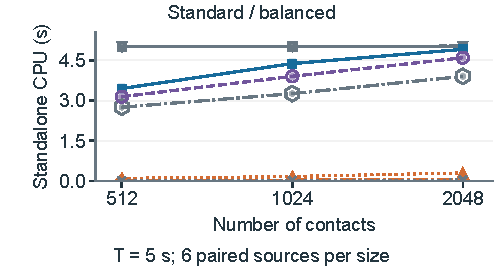
\includegraphics[width=\linewidth]{figures/performance_cpu_scaling_v06__fresh_standard_balanced__standard_balanced.pdf}
    {\small (a)}
  \end{minipage}\hfill
  \begin{minipage}[t]{0.495\textwidth}
    \centering
    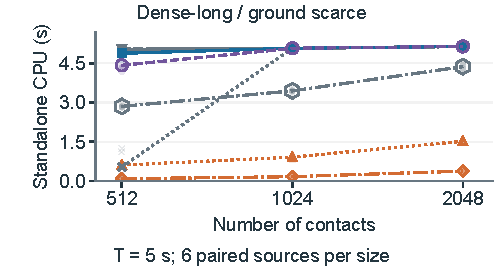
\includegraphics[width=\linewidth]{figures/performance_cpu_scaling_v06__fresh_dense_long_ground_scarce__dense_long_ground_scarce.pdf}
    {\small (b)}
  \end{minipage}
  \par\vspace{1pt}
  
\includegraphics[width=\textwidth]{figures/performance_cpu_scaling_legend_v06.pdf}
  \caption{Measured deployment CPU versus contact count at fixed nominal
  $T=5$ seconds: standard balanced (a) and dense-long ground scarce (b).
  Faint points show six paired sources per size; lines show their mean,
  after within-context seed/member averaging. Warm policies each charge
  the full common CHILS initializer and their own repair; shared graph
  loading remains separate. These are scale comparisons, not anytime traces
  or evidence of LLM speed superiority. Complete gain/coverage matrices
  remain in the supporting report.}
  \Description{Two panels compare actual standalone CPU seconds at contact
  counts 512, 1024, and 2048 for five native method families and warm
  joint witness, EoH-DSL, and Degree policies. Each faint point is one
  paired-source cost; each line joins the six-source means at the three
  sizes. All policies use their frozen identities and native methods
  retain their prescribed seeds. A shared legend identifies eight curves.
  The comparison uses fixed nominal five-second targets and retains
  the full charged common initializer for warm policies.}
  \label{fig:v06_performance_budget}
\end{figure*}
}{}
